\let\negmedspace\undefined
\let\negthickspace\undefined
\documentclass[journal,12pt,onecolumn]{IEEEtran}
\usepackage{cite}
\usepackage{amsmath,amssymb,amsfonts,amsthm}
\usepackage{algorithmic}
\usepackage{graphicx}
\usepackage{textcomp}
\usepackage{xcolor}
\usepackage{txfonts}
\usepackage{listings}
\usepackage{enumitem}
\usepackage{mathtools}
\usepackage{gensymb}
\usepackage{comment}
\usepackage[breaklinks=true]{hyperref}
\usepackage{tkz-euclide} 
\usepackage{listings}
\usepackage{gvv}                                        
%\def\inputGnumericTable{}                                 
\usepackage[latin1]{inputenc}                                
\usepackage{color}                                            
\usepackage{array}                                            
\usepackage{longtable}                                       
\usepackage{calc}   
\usepackage{multicol}
\usepackage{multirow}                                         
\usepackage{hhline}                                           
\usepackage{ifthen}                                           
\usepackage{lscape}
\usepackage{tabularx}
\usepackage{array}
\usepackage{float}
\usepackage{circuitikz}

\newtheorem{theorem}{Theorem}[section]
\newtheorem{problem}{Problem}
\newtheorem{proposition}{Proposition}[section]
\newtheorem{lemma}{Lemma}[section]
\newtheorem{corollary}[theorem]{Corollary}
\newtheorem{example}{Example}[section]
\newtheorem{definition}[problem]{Definition}
\newcommand{\BEQA}{\begin{eqnarray}}
\newcommand{\nCr}[2]{\,^{#1}C_{#2}}
\newcommand{\EEQA}{\end{eqnarray}}

\begin{document}
\vspace{3cm}
\title{DIGITAL THERMOMETER USING PT-100}
\author{Harsha B J and Bhargav K}
\maketitle

\newpage
\tableofcontents

\newpage
\bigskip

\section{\textbf{Objective}}
The objective of this project is to design and implement a digital thermometer that measures the temperature using a PT-100 Resistance Temperature Detector (RTD), processes the signal through an Arduino microcontroller, and displays the temperature on a 16$\times$2 LCD. In this experiment, the relationship between the voltage across
the PT-100 and the temperature is determined using linear regression (least squares
method).

\section{\textbf{Training Data}}
The training data gathered by the PT-100 to train the Arduino is shown in Table
\ref{tab:train}.

\begin{table}[H]
    \centering
    %%%%%%%%%%%%%%%%%%%%%%%%%%%%%%%%%%%%%%%%%%%%%%%%%%%%%%%%%%%%%%%%%%%%%%
%%                                                     %%
%%  This is the header of a LaTeX2e file exported from Gnumeric.    %%
%%                                                     %%
%%  This file can be compiled as it stands or included in another   %%
%%  LaTeX document. The table is based on the longtable package so  %%
%%  the longtable options (headers, footers...) can be set in the   %%
%%  preamble section below (see PRAMBLE).                      %%
%%                                                     %%
%%  To include the file in another, the following two lines must be %%
%%  in the including file:                                  %%
%%       \def\inputGnumericTable{}                           %%
%%  at the beginning of the file and:                         %%
%%       \input{name-of-this-file.tex}                        %%
%%  where the table is to be placed. Note also that the including   %%
%%  file must use the following packages for the table to be       %%
%%  rendered correctly:                                    %%
%%    \usepackage[latin1]{inputenc}                           %%
%%    \usepackage{color}                                    %%
%%    \usepackage{array}                                    %%
%%    \usepackage{longtable}                                %%
%%    \usepackage{calc}                                    %%
%%    \usepackage{multirow}                                 %%
%%    \usepackage{hhline}                                   %%
%%    \usepackage{ifthen}                                   %%
%%  optionally (for landscape tables embedded in another document): %%
%%    \usepackage{lscape}                                   %%
%%                                                     %%
%%%%%%%%%%%%%%%%%%%%%%%%%%%%%%%%%%%%%%%%%%%%%%%%%%%%%%%%%%%%%%%%%%%%%%



%%  This section checks if we are begin input into another file or  %%
%%  the file will be compiled alone. First use a macro taken from   %%
%%  the TeXbook ex 7.7 (suggestion of Han-Wen Nienhuys).          %%
\def\ifundefined#1{\expandafter\ifx\csname#1\endcsname\relax}


%%  Check for the \def token for inputed files. If it is not       %%
%%  defined, the file will be processed as a standalone and the    %%
%%  preamble will be used.                                  %%
\ifundefined{inputGnumericTable}

%%  We must be able to close or not the document at the end.       %%
	\def\gnumericTableEnd{\end{document}}


%%%%%%%%%%%%%%%%%%%%%%%%%%%%%%%%%%%%%%%%%%%%%%%%%%%%%%%%%%%%%%%%%%%%%%
%%                                                     %%
%%  This is the PREAMBLE. Change these values to get the right     %%
%%  paper size and other niceties.                            %%
%%                                                     %%
%%%%%%%%%%%%%%%%%%%%%%%%%%%%%%%%%%%%%%%%%%%%%%%%%%%%%%%%%%%%%%%%%%%%%%

	\documentclass[12pt%
			  %,landscape%
                ]{report}
      \usepackage[latin1]{inputenc}
      \usepackage{fullpage}
      \usepackage{color}
      \usepackage{array}
      \usepackage{longtable}
      \usepackage{calc}
      \usepackage{multirow}
      \usepackage{hhline}
      \usepackage{ifthen}

	\begin{document}


%%  End of the preamble for the standalone. The next section is for %%
%%  documents which are included into other LaTeX2e files.        %%
\else

%%  We are not a stand alone document. For a regular table, we will %%
%%  have no preamble and only define the closing to mean nothing.   %%
    \def\gnumericTableEnd{}

%%  If we want landscape mode in an embedded document, comment out  %%
%%  the line above and uncomment the two below. The table will     %%
%%  begin on a new page and run in landscape mode.               %%
%      \def\gnumericTableEnd{\end{landscape}}
%      \begin{landscape}


%%  End of the else clause for this file being \input.            %%
\fi

%%%%%%%%%%%%%%%%%%%%%%%%%%%%%%%%%%%%%%%%%%%%%%%%%%%%%%%%%%%%%%%%%%%%%%
%%                                                     %%
%%  The rest is the gnumeric table, except for the closing        %%
%%  statement. Changes below will alter the table's appearance.    %%
%%                                                     %%
%%%%%%%%%%%%%%%%%%%%%%%%%%%%%%%%%%%%%%%%%%%%%%%%%%%%%%%%%%%%%%%%%%%%%%

\providecommand{\gnumericmathit}[1]{#1} 
%%  Uncomment the next line if you would like your numbers to be in %%
%%  italics if they are italizised in the gnumeric table.         %%
%\renewcommand{\gnumericmathit}[1]{\mathit{#1}}
\providecommand{\gnumericPB}[1]%
{\let\gnumericTemp=\\#1\let\\=\gnumericTemp\hspace{0pt}}
 \ifundefined{gnumericTableWidthDefined}
       \newlength{\gnumericTableWidth}
       \newlength{\gnumericTableWidthComplete}
       \newlength{\gnumericMultiRowLength}
       \global\def\gnumericTableWidthDefined{}
 \fi
%% The following setting protects this code from babel shorthands.  %%
 \ifthenelse{\isundefined{\languageshorthands}}{}{\languageshorthands{english}}
%%  The default table format retains the relative column widths of  %%
%%  gnumeric. They can easily be changed to c, r or l. In that case %%
%%  you may want to comment out the next line and uncomment the one %%
%%  thereafter                                            %%
\providecommand\gnumbox{\makebox[0pt]}
%%\providecommand\gnumbox[1][]{\makebox}

%% to adjust positions in multirow situations                   %%
\setlength{\bigstrutjot}{\jot}
\setlength{\extrarowheight}{\doublerulesep}

%%  The \setlongtables command keeps column widths the same across  %%
%%  pages. Simply comment out next line for varying column widths.  %%
\setlongtables

\setlength\gnumericTableWidth{%
	101pt+%
	69pt+%
	67pt+%
0pt}
\def\gumericNumCols{3}
\setlength\gnumericTableWidthComplete{\gnumericTableWidth+%
        \tabcolsep*\gumericNumCols*2+\arrayrulewidth*\gumericNumCols}
\ifthenelse{\lengthtest{\gnumericTableWidthComplete > \linewidth}}%
        {\def\gnumericScale{1*\ratio{\linewidth-%
                    \tabcolsep*\gumericNumCols*2-%
                    \arrayrulewidth*\gumericNumCols}%
{\gnumericTableWidth}}}%
{\def\gnumericScale{1}}

%%%%%%%%%%%%%%%%%%%%%%%%%%%%%%%%%%%%%%%%%%%%%%%%%%%%%%%%%%%%%%%%%%%%%%
%%                                                     %%
%% The following are the widths of the various columns. We are     %%
%% defining them here because then they are easier to change.      %%
%% Depending on the cell formats we may use them more than once.    %%
%%                                                     %%
%%%%%%%%%%%%%%%%%%%%%%%%%%%%%%%%%%%%%%%%%%%%%%%%%%%%%%%%%%%%%%%%%%%%%%

\ifthenelse{\isundefined{\gnumericColA}}{\newlength{\gnumericColA}}{}\settowidth{\gnumericColA}{\begin{tabular}{@{}p{101pt*\gnumericScale}@{}}x\end{tabular}}
\ifthenelse{\isundefined{\gnumericColB}}{\newlength{\gnumericColB}}{}\settowidth{\gnumericColB}{\begin{tabular}{@{}p{69pt*\gnumericScale}@{}}x\end{tabular}}
\ifthenelse{\isundefined{\gnumericColC}}{\newlength{\gnumericColC}}{}\settowidth{\gnumericColC}{\begin{tabular}{@{}p{67pt*\gnumericScale}@{}}x\end{tabular}}

\begin{tabular}[c]{%
	b{\gnumericColA}%
	b{\gnumericColB}%
	b{\gnumericColC}%
	}

%%%%%%%%%%%%%%%%%%%%%%%%%%%%%%%%%%%%%%%%%%%%%%%%%%%%%%%%%%%%%%%%%%%%%%
%%  The longtable options. (Caption, headers... see Goosens, p.124) %%
%	\caption{The Table Caption.}           \\	%
% \hline	% Across the top of the table.
%%  The rest of these options are table rows which are placed on    %%
%%  the first, last or every page. Use \multicolumn if you want.    %%

%%  Header for the first page.                               %%
%	\multicolumn{3}{c}{The First Header} \\ \hline 
%	\multicolumn{1}{c}{colTag}	%Column 1
%	&\multicolumn{1}{c}{colTag}	%Column 2
%	&\multicolumn{1}{c}{colTag}	\\ \hline %Last column
%	\endfirsthead

%%  The running header definition.                            %%
%	\hline
%	\multicolumn{3}{l}{\ldots\small\slshape continued} \\ \hline
%	\multicolumn{1}{c}{colTag}	%Column 1
%	&\multicolumn{1}{c}{colTag}	%Column 2
%	&\multicolumn{1}{c}{colTag}	\\ \hline %Last column
%	\endhead

%%  The running footer definition.                            %%
%	\hline
%	\multicolumn{3}{r}{\small\slshape continued\ldots} \\
%	\endfoot

%%  The ending footer definition.                            %%
%	\multicolumn{3}{c}{That's all folks} \\ \hline 
%	\endlastfoot
%%%%%%%%%%%%%%%%%%%%%%%%%%%%%%%%%%%%%%%%%%%%%%%%%%%%%%%%%%%%%%%%%%%%%%

\hhline{|-|-~}
	 \multicolumn{1}{|p{\gnumericColA}|}%
    {\gnumericPB{\raggedright}\gnumbox[l]{\textbf{Temperature ($^{\circ}$C)}}}
	&\multicolumn{1}{p{\gnumericColB}|}%
	{\gnumericPB{\raggedright}\gnumbox[l]{\textbf{Voltage (V)}}}
	&

\\
\hhline{|-|-~}
	 \multicolumn{1}{|p{\gnumericColA}|}%
    {\gnumericPB{\raggedright}\gnumbox[l]{25.00}}
	&\multicolumn{1}{p{\gnumericColB}|}%
	{\gnumericPB{\raggedright}\gnumbox[l]{2.834}}
	&
\\

\hhline{|-|-~}
	 \multicolumn{1}{|p{\gnumericColA}|}%
    {\gnumericPB{\raggedright}\gnumbox[l]{31.31}}
	&\multicolumn{1}{p{\gnumericColB}|}%
	{\gnumericPB{\raggedright}\gnumbox[l]{2.856}}
	&
\\
\hhline{|-|-~}
	 \multicolumn{1}{|p{\gnumericColA}|}%
    {\gnumericPB{\raggedright}\gnumbox[l]{34.46}}
	&\multicolumn{1}{p{\gnumericColB}|}%
	{\gnumericPB{\raggedright}\gnumbox[l]{2.868}}
	&
\\
\hhline{|-|-~}
	 \multicolumn{1}{|p{\gnumericColA}|}%
    {\gnumericPB{\raggedright}\gnumbox[l]{37.61}}
	&\multicolumn{1}{p{\gnumericColB}|}%
	{\gnumericPB{\raggedright}\gnumbox[l]{2.879}}
	&
\\
\hhline{|-|-~}
	 \multicolumn{1}{|p{\gnumericColA}|}%
    {\gnumericPB{\raggedright}\gnumbox[l]{40.76}}
	&\multicolumn{1}{p{\gnumericColB}|}%
	{\gnumericPB{\raggedright}\gnumbox[l]{2.890}}
	&
\\

\hhline{|-|-~}
	 \multicolumn{1}{|p{\gnumericColA}|}%
    {\gnumericPB{\raggedright}\gnumbox[l]{47.07}}
	&\multicolumn{1}{p{\gnumericColB}|}%
	{\gnumericPB{\raggedright}\gnumbox[l]{2.912}}
	&
\\
\hhline{|-|-~}
	 \multicolumn{1}{|p{\gnumericColA}|}%
    {\gnumericPB{\raggedright}\gnumbox[l]{50.22}}
	&\multicolumn{1}{p{\gnumericColB}|}%
	{\gnumericPB{\raggedright}\gnumbox[l]{2.924}}
	&
\\
\hhline{|-|-~}
	 \multicolumn{1}{|p{\gnumericColA}|}%
    {\gnumericPB{\raggedright}\gnumbox[l]{53.37}}
	&\multicolumn{1}{p{\gnumericColB}|}%
	{\gnumericPB{\raggedright}\gnumbox[l]{2.935}}
	&
\\

\hhline{|-|-~}
	 \multicolumn{1}{|p{\gnumericColA}|}%
    {\gnumericPB{\raggedright}\gnumbox[l]{59.68}}
	&\multicolumn{1}{p{\gnumericColB}|}%
	{\gnumericPB{\raggedright}\gnumbox[l]{2.957}}
	&
\\
\hhline{|-|-~}
	 \multicolumn{1}{|p{\gnumericColA}|}%
    {\gnumericPB{\raggedright}\gnumbox[l]{62.83}}
	&\multicolumn{1}{p{\gnumericColB}|}%
	{\gnumericPB{\raggedright}\gnumbox[l]{2.968}}
	&
\\
\hhline{|-|-~}
	 \multicolumn{1}{|p{\gnumericColA}|}%
    {\gnumericPB{\raggedright}\gnumbox[l]{65.98}}
	&\multicolumn{1}{p{\gnumericColB}|}%
	{\gnumericPB{\raggedright}\gnumbox[l]{2.980}}
	&
\\

\hhline{|-|-~}
	 \multicolumn{1}{|p{\gnumericColA}|}%
    {\gnumericPB{\raggedright}\gnumbox[l]{72.29}}
	&\multicolumn{1}{p{\gnumericColB}|}%
	{\gnumericPB{\raggedright}\gnumbox[l]{3.002}}
	&
\\
\hhline{|-|-~}
	 \multicolumn{1}{|p{\gnumericColA}|}%
    {\gnumericPB{\raggedright}\gnumbox[l]{75.44}}
	&\multicolumn{1}{p{\gnumericColB}|}%
	{\gnumericPB{\raggedright}\gnumbox[l]{3.013}}
	&
\\
\hhline{|-|-~}
	 \multicolumn{1}{|p{\gnumericColA}|}%
    {\gnumericPB{\raggedright}\gnumbox[l]{78.59}}
	&\multicolumn{1}{p{\gnumericColB}|}%
	{\gnumericPB{\raggedright}\gnumbox[l]{3.024}}
	&
\\

\hhline{|-|-~}
	 \multicolumn{1}{|p{\gnumericColA}|}%
    {\gnumericPB{\raggedright}\gnumbox[l]{84.90}}
	&\multicolumn{1}{p{\gnumericColB}|}%
	{\gnumericPB{\raggedright}\gnumbox[l]{3.047}}
	&
\\
\hhline{|-|-~}
\end{tabular}

\ifthenelse{\isundefined{\languageshorthands}}{}{\languageshorthands{\languagename}}
\gnumericTableEnd

    \caption{Training data.}
    \label{tab:train}
\end{table}

The C++ source \texttt{codes/data.cpp} was used along with \textit{platformio} to drive the Arduino.

The approximation is shown in Fig. \ref{fig:train}.
\begin{figure}[H]
    \centering
    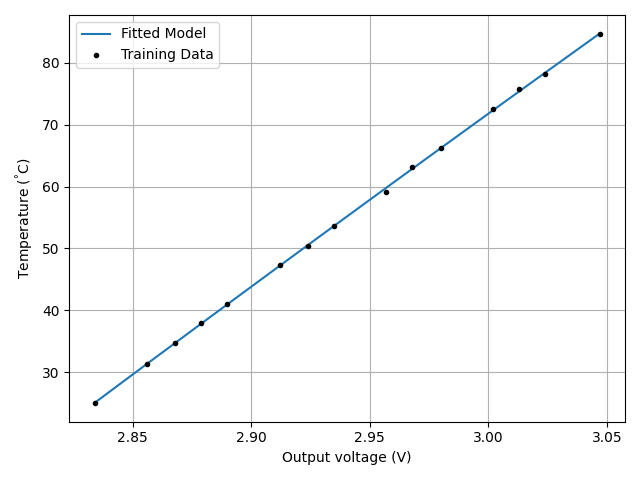
\includegraphics[width=0.6\columnwidth]{figs/temp_vs_voltage/train.png}
    \label{fig:train}
\end{figure}

\vspace{2cm}

\section{\textbf{Theory}}
The PT-100 sensor changes resistance with temperature. Its nominal resistance is 100 $\ohm$
at 0 $\degree$C, and the resistance increases approximately linearly with temperature:
\begin{align}
R_T = R_o(1 + \alpha T)
\end{align}
where $\alpha$ = 0.00385 $\degree C^{-1}$. When placed in a Wheatstone bridge circuit, the resistance variation produces a corresponding voltage change, which can be measured and used to infer the temperature.


\section{\textbf{Linear Regression Model}}
To obtain an empirical model relating the measured voltage V to temperature T, we collect calibration data by measuring both quantities over a range of known temperatures. Let the measured data points be ($T_i$ , $V_i$), i = 1, 2,. . , n. We assume a quadratic model for the voltage-temperature relationship
\begin{align}
    V(T) &= n_0+n_1T+n_2T^2 \\
\end{align}
\begin{align}
    \implies \vec{C} = \vec{X^T}\vec{n}  \label{eq:model}
\end{align}
where
\begin{align}
   \vec{X^T} = \myvec{1 & T_1 & T_1^2 \\ 1 & T_2 & T_2^2 \\ . & . & .\\ . & . & .\\ . & . & . \\ 1 & T_n & T_n^2}, \vec{C} = \myvec{V_1 \\ V_2 \\ . \\ . \\ . \\ V_n}
    \label{eq:x-y-theta-def}
\end{align}



\section{\textbf{Solution}}
We approximate $\vec{n^T} = \myvec{n_0 & n_1 & n_2}$ using the least squares method. Using the pseudo-inverse method, the solution to \eqref{eq:model} is
\begin{align}
    \vec{n} = \brak{\vec{XX}^\top}^{-1}\vec{X}\vec{C}
\end{align}
The Python code \texttt{codes/main.py} solves for $\vec{n}$.
The calculated value of $\vec{n}$ is
\begin{align}
    \vec{n} = \myvec{2.7451\\3.5566\times10^{-3}\\-5.0234\times10^{-8}}
    \label{eq:opt-theta-1}
\end{align}
To obtain temperature as a function of measured voltage (for Arduino implementation), we rearrange or numerically invert the above relation:
\begin{align}
T(V) = a_0 + a_1V + a_2V^2
\end{align}
The coefficients $a_i$ can again be found by applying the least squares method to the ($V_i$, $T_i$)
data, which yields
\begin{align}
    \vec{n} = \myvec{-996.9724\\435.5577\\-26.4382}
    \label{eq:opt-theta-2}
\end{align}


\section{\textbf{Validation}}
The validation data set is shown in Table \ref{tab:valid}. The results of the
validation are shown in Fig. \ref{fig:valid}.
\begin{table}[H]
    \centering
    %%%%%%%%%%%%%%%%%%%%%%%%%%%%%%%%%%%%%%%%%%%%%%%%%%%%%%%%%%%%%%%%%%%%%%
%%                                                                  %%
%%  This is the header of a LaTeX2e file exported from Gnumeric.    %%
%%                                                                  %%
%%  This file can be compiled as it stands or included in another   %%
%%  LaTeX document. The table is based on the longtable package so  %%
%%  the longtable options (headers, footers...) can be set in the   %%
%%  preamble section below (see PRAMBLE).                           %%
%%                                                                  %%
%%  To include the file in another, the following two lines must be %%
%%  in the including file:                                          %%
%%        \def\inputGnumericTable{}                                 %%
%%  at the beginning of the file and:                               %%
%%        \input{name-of-this-file.tex}                             %%
%%  where the table is to be placed. Note also that the including   %%
%%  file must use the following packages for the table to be        %%
%%  rendered correctly:                                             %%
%%    \usepackage[latin1]{inputenc}                                 %%
%%    \usepackage{color}                                            %%
%%    \usepackage{array}                                            %%
%%    \usepackage{longtable}                                        %%
%%    \usepackage{calc}                                             %%
%%    \usepackage{multirow}                                         %%
%%    \usepackage{hhline}                                           %%
%%    \usepackage{ifthen}                                           %%
%%  optionally (for landscape tables embedded in another document): %%
%%    \usepackage{lscape}                                           %%
%%                                                                  %%
%%%%%%%%%%%%%%%%%%%%%%%%%%%%%%%%%%%%%%%%%%%%%%%%%%%%%%%%%%%%%%%%%%%%%%



%%  This section checks if we are begin input into another file or  %%
%%  the file will be compiled alone. First use a macro taken from   %%
%%  the TeXbook ex 7.7 (suggestion of Han-Wen Nienhuys).            %%
\def\ifundefined#1{\expandafter\ifx\csname#1\endcsname\relax}


%%  Check for the \def token for inputed files. If it is not        %%
%%  defined, the file will be processed as a standalone and the     %%
%%  preamble will be used.                                          %%
\ifundefined{inputGnumericTable}

%%  We must be able to close or not the document at the end.        %%
	\def\gnumericTableEnd{\end{document}}


%%%%%%%%%%%%%%%%%%%%%%%%%%%%%%%%%%%%%%%%%%%%%%%%%%%%%%%%%%%%%%%%%%%%%%
%%                                                                  %%
%%  This is the PREAMBLE. Change these values to get the right      %%
%%  paper size and other niceties.                                  %%
%%                                                                  %%
%%%%%%%%%%%%%%%%%%%%%%%%%%%%%%%%%%%%%%%%%%%%%%%%%%%%%%%%%%%%%%%%%%%%%%

	\documentclass[12pt%
			  %,landscape%
                    ]{report}
       \usepackage[latin1]{inputenc}
       \usepackage{fullpage}
       \usepackage{color}
       \usepackage{array}
       \usepackage{longtable}
       \usepackage{calc}
       \usepackage{multirow}
       \usepackage{hhline}
       \usepackage{ifthen}




%%  End of the preamble for the standalone. The next section is for %%
%%  documents which are included into other LaTeX2e files.          %%
\else

%%  We are not a stand alone document. For a regular table, we will %%
%%  have no preamble and only define the closing to mean nothing.   %%
    \def\gnumericTableEnd{}

%%  If we want landscape mode in an embedded document, comment out  %%
%%  the line above and uncomment the two below. The table will      %%
%%  begin on a new page and run in landscape mode.                  %%
%       \def\gnumericTableEnd{\end{landscape}}
%       \begin{landscape}


%%  End of the else clause for this file being \input.              %%
\fi

%%%%%%%%%%%%%%%%%%%%%%%%%%%%%%%%%%%%%%%%%%%%%%%%%%%%%%%%%%%%%%%%%%%%%%
%%                                                                  %%
%%  The rest is the gnumeric table, except for the closing          %%
%%  statement. Changes below will alter the table's appearance.     %%
%%                                                                  %%
%%%%%%%%%%%%%%%%%%%%%%%%%%%%%%%%%%%%%%%%%%%%%%%%%%%%%%%%%%%%%%%%%%%%%%

\providecommand{\gnumericmathit}[1]{#1} 
%%  Uncomment the next line if you would like your numbers to be in %%
%%  italics if they are italizised in the gnumeric table.           %%
%\renewcommand{\gnumericmathit}[1]{\mathit{#1}}
\providecommand{\gnumericPB}[1]%
{\let\gnumericTemp=\\#1\let\\=\gnumericTemp\hspace{0pt}}
 \ifundefined{gnumericTableWidthDefined}
        \newlength{\gnumericTableWidth}
        \newlength{\gnumericTableWidthComplete}
        \newlength{\gnumericMultiRowLength}
        \global\def\gnumericTableWidthDefined{}
 \fi
%% The following setting protects this code from babel shorthands.  %%
 \ifthenelse{\isundefined{\languageshorthands}}{}{\languageshorthands{english}}
%%  The default table format retains the relative column widths of  %%
%%  gnumeric. They can easily be changed to c, r or l. In that case %%
%%  you may want to comment out the next line and uncomment the one %%
%%  thereafter                                                      %%
\providecommand\gnumbox{\makebox[0pt]}
%%\providecommand\gnumbox[1][]{\makebox}

%% to adjust positions in multirow situations                       %%
\setlength{\bigstrutjot}{\jot}
\setlength{\extrarowheight}{\doublerulesep}

%%  The \setlongtables command keeps column widths the same across  %%
%%  pages. Simply comment out next line for varying column widths.  %%
\setlongtables

\setlength\gnumericTableWidth{%
	101pt+%
	69pt+%
	67pt+%
0pt}
\def\gumericNumCols{3}
\setlength\gnumericTableWidthComplete{\gnumericTableWidth+%
         \tabcolsep*\gumericNumCols*2+\arrayrulewidth*\gumericNumCols}
\ifthenelse{\lengthtest{\gnumericTableWidthComplete > \linewidth}}%
         {\def\gnumericScale{1*\ratio{\linewidth-%
                        \tabcolsep*\gumericNumCols*2-%
                        \arrayrulewidth*\gumericNumCols}%
{\gnumericTableWidth}}}%
{\def\gnumericScale{1}}

%%%%%%%%%%%%%%%%%%%%%%%%%%%%%%%%%%%%%%%%%%%%%%%%%%%%%%%%%%%%%%%%%%%%%%
%%                                                                  %%
%% The following are the widths of the various columns. We are      %%
%% defining them here because then they are easier to change.       %%
%% Depending on the cell formats we may use them more than once.    %%
%%                                                                  %%
%%%%%%%%%%%%%%%%%%%%%%%%%%%%%%%%%%%%%%%%%%%%%%%%%%%%%%%%%%%%%%%%%%%%%%

\ifthenelse{\isundefined{\gnumericColA}}{\newlength{\gnumericColA}}{}\settowidth{\gnumericColA}{\begin{tabular}{@{}p{101pt*\gnumericScale}@{}}x\end{tabular}}
\ifthenelse{\isundefined{\gnumericColB}}{\newlength{\gnumericColB}}{}\settowidth{\gnumericColB}{\begin{tabular}{@{}p{69pt*\gnumericScale}@{}}x\end{tabular}}
\ifthenelse{\isundefined{\gnumericColC}}{\newlength{\gnumericColC}}{}\settowidth{\gnumericColC}{\begin{tabular}{@{}p{67pt*\gnumericScale}@{}}x\end{tabular}}

\begin{tabular}[c]{%
	b{\gnumericColA}%
	b{\gnumericColB}%
	b{\gnumericColC}%
	}

%%%%%%%%%%%%%%%%%%%%%%%%%%%%%%%%%%%%%%%%%%%%%%%%%%%%%%%%%%%%%%%%%%%%%%
%%  The longtable options. (Caption, headers... see Goosens, p.124) %%
%	\caption{The Table Caption.}             \\	%
% \hline	% Across the top of the table.
%%  The rest of these options are table rows which are placed on    %%
%%  the first, last or every page. Use \multicolumn if you want.    %%

%%  Header for the first page.                                      %%
%	\multicolumn{3}{c}{The First Header} \\ \hline 
%	\multicolumn{1}{c}{colTag}	%Column 1
%	&\multicolumn{1}{c}{colTag}	%Column 2
%	&\multicolumn{1}{c}{colTag}	\\ \hline %Last column
%	\endfirsthead

%%  The running header definition.                                  %%
%	\hline
%	\multicolumn{3}{l}{\ldots\small\slshape continued} \\ \hline
%	\multicolumn{1}{c}{colTag}	%Column 1
%	&\multicolumn{1}{c}{colTag}	%Column 2
%	&\multicolumn{1}{c}{colTag}	\\ \hline %Last column
%	\endhead

%%  The running footer definition.                                  %%
%	\hline
%	\multicolumn{3}{r}{\small\slshape continued\ldots} \\
%	\endfoot

%%  The ending footer definition.                                   %%
%	\multicolumn{3}{c}{That's all folks} \\ \hline 
%	\endlastfoot
%%%%%%%%%%%%%%%%%%%%%%%%%%%%%%%%%%%%%%%%%%%%%%%%%%%%%%%%%%%%%%%%%%%%%%


\hhline{|-|-~}
	 \multicolumn{1}{|p{\gnumericColA}|}%
     {\gnumericPB{\raggedright}\gnumbox[l]{\textbf{Temperature ($^{\circ}$C)}}}
	&\multicolumn{1}{p{\gnumericColB}|}%
	{\gnumericPB{\raggedright}\gnumbox[l]{\textbf{Voltage (V)}}}
	&
\\
\hhline{|-|-~}
	 \multicolumn{1}{|p{\gnumericColA}|}%
    {\gnumericPB{\raggedright}\gnumbox[l]{28.15}}
	&\multicolumn{1}{p{\gnumericColB}|}%
	{\gnumericPB{\raggedright}\gnumbox[l]{2.845}}
	&
\\
\hhline{|-|-~}
	 \multicolumn{1}{|p{\gnumericColA}|}%
    {\gnumericPB{\raggedright}\gnumbox[l]{43.92}}
	&\multicolumn{1}{p{\gnumericColB}|}%
	{\gnumericPB{\raggedright}\gnumbox[l]{2.901}}
	&

\\
\hhline{|-|-~}
	 \multicolumn{1}{|p{\gnumericColA}|}%
    {\gnumericPB{\raggedright}\gnumbox[l]{56.53}}
	&\multicolumn{1}{p{\gnumericColB}|}%
	{\gnumericPB{\raggedright}\gnumbox[l]{2.946}}
	&
\\
\hhline{|-|-~}
	 \multicolumn{1}{|p{\gnumericColA}|}%
    {\gnumericPB{\raggedright}\gnumbox[l]{69.14}}
	&\multicolumn{1}{p{\gnumericColB}|}%
	{\gnumericPB{\raggedright}\gnumbox[l]{2.991}}
	&
\\
\hhline{|-|-~}
	 \multicolumn{1}{|p{\gnumericColA}|}%
    {\gnumericPB{\raggedright}\gnumbox[l]{81.75}}
	&\multicolumn{1}{p{\gnumericColB}|}%
	{\gnumericPB{\raggedright}\gnumbox[l]{3.036}}
	&
\\

\hhline{|-|-|~}
\end{tabular}

\ifthenelse{\isundefined{\languageshorthands}}{}{\languageshorthands{\languagename}}
\gnumericTableEnd

    \caption{Validation data.}
    \label{tab:valid}
\end{table}
\begin{figure}[H]
    \centering
    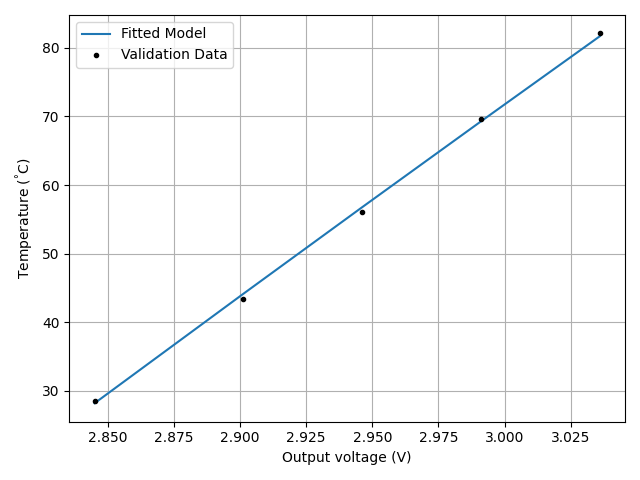
\includegraphics[width=0.6\columnwidth]{figs/temp_vs_voltage/valid.png}
    \label{fig:valid}
\end{figure}

\section{\textbf{Conceptual logic implemented in the code}}
The provided program implements a quadratic regression model to establish the relationship between temperature and output voltage. It begins by loading the training data consisting of temperature (in $\degree$C) and voltage (in V) readings. A design matrix is then constructed using three terms: a constant, the temperature, and the square of the temperature. By applying the least squares method, the program determines the model coefficients that best fit the data. This fitted model is then used to generate predicted voltage values, which are plotted against the actual training data to visualize the accuracy of the fit.\\
\\
Subsequently, the program loads a separate validation dataset to evaluate the performance of the derived model on unseen data. The fitted curve and the actual validation data points are plotted together, allowing a clear comparison of the predicted and measured values. The resulting plots are saved for documentation, and the computed model parameters are printed for further analysis. In essence, the code effectively demonstrates the use of polynomial regression for sensor calibration and performance verification.

\section{\textbf{Observation}}
The observations made while conducting the experiment are as follows,
\begin{enumerate}
    \item The readings of arduino had an offset of a few millivolts for every cycle of reading.
    Solution: We wrote an algorithm to take an average of a few sample readings and computed the temperature using it which gave a good precision.
    \item The values of the temperature had an offset of $\pm \,3\degree$ celcius due to the hardware \\malfunctioning.
    \item the accuracy of the training model and validation data is close enough with a less validation.
\end{enumerate}


\section{\textbf{Circuit Diagram}}
\begin{figure}[H]
    \centering
    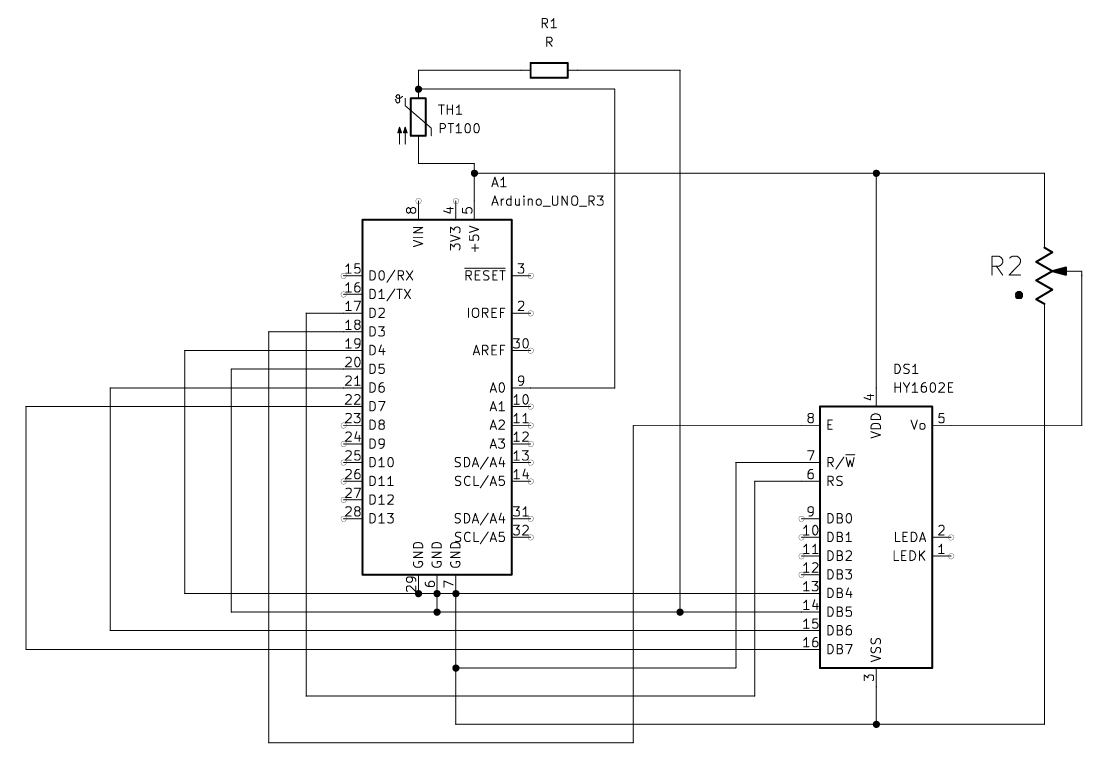
\includegraphics[width=0.8\columnwidth]{figs/circuit diagram.jpeg}
    \label{fig:crtdiagram}
\end{figure}



\section{\textbf{Conclusion}}

This project used Python for machine learning to calibrate the temperature sensor with linear regression. Arduino collected sensor data and showed real-time results. Python made the analysis easier and more accurate, while Arduino handled the hardware side. This simple combination of Python and Arduino creates a smart, affordable device by merging data science and embedded systems effectively.


\end{document}
